\documentclass[12pt, a4paper]{mwart}

\usepackage[utf8]{inputenc}								%kodowanie znaków
\usepackage[T1]{fontenc}								%kodowanie fontu
\usepackage{polski}										%polskie wcięcia itp
\usepackage{graphicx}									%wstawianie grafik
\usepackage{booktabs}									%scalanie kolumn
\usepackage{enumitem}									%lista a), b), c)
\usepackage{multirow}									%scalanie komórek tabeli w pionie
\usepackage{listings}									%wklejanie kodu z SQL
\usepackage{xcolor}										%żeby kolory do kodu działaly
\usepackage[margin=0.5in]{geometry}						%zmiana marginesów
\usepackage[hidelinks]{hyperref}						%linki w spisie treści

\usepackage{verbatim}									%multi-line comment
%\usepackage{tocloft}									%change spacing in table of contents
%\setlength{\cftfignumwidth}{2.55em}

\hypersetup{linktoc=all}								%ustawienie linków w spisie treści
\linespread{1.3}										%interlinia 1,5

\lstset{ %
  backgroundcolor=\color{white},   % choose the background color; you must add \usepackage{color} or \usepackage{xcolor}; should come as last argument
  basicstyle=\scriptsize,        % the size of the fonts that are used for the code
  breakatwhitespace=false,         % sets if automatic breaks should only happen at whitespace
  breaklines=true,                 % sets automatic line breaking
  commentstyle=\color{gray},       % comment style
  extendedchars=true,              % lets you use non-ASCII characters; for 8-bits encodings only, does not work with UTF-8
  frame=single,	                   % adds a frame around the code
  language=java,
  keywordstyle=\color{blue},       % keyword style
  morekeywords={*,...},            % if you want to add more keywords to the set
  numbers=left,                    % where to put the line-numbers; possible values are (none, left, right)
  numbersep=5pt,                   % how far the line-numbers are from the code
  numberstyle=\normalsize,			% the style that is used for the line-numbers
  rulecolor=\color{black},         % if not set, the frame-color may be changed on line-breaks within not-black text (e.g. comments (green here))
  showspaces=false,                % show spaces everywhere adding particular underscores; it overrides 'showstringspaces'
  showstringspaces=false,          % underline spaces within strings only
  showtabs=false,                  % show tabs within strings adding particular underscores
  stepnumber=1,                    % the step between two line-numbers. If it's 1, each line will be numbered
  stringstyle=\color{orange},      % string literal style
  tabsize=2	                   	   % sets default tabsize to 2 spaces                   
}

\lstset{
literate=%
{ą}{{\k{a}}}1
{Ą}{{\k{A}}}1
{ć}{{\'c}}1
{Ć}{{\'{C}}}1
{ę}{{\k{e}}}1
{Ę}{{\k{E}}}1
{ł}{{\l{}}}1
{Ł}{{\L{}}}1
{ń}{{\'n}}1
{Ń}{{\'N}}1
{ó}{{\'o}}1
{Ó}{{\'O}}1
{ś}{{\'s}}1
{Ś}{{\'S}}1
{ż}{{\.z}}1
{Ż}{{\.Z}}1
{ź}{{\'z}}1
{Ź}{{\'Z}}1
}

\begin{document}

\begin{center}
Piotr Wróbel

Hibernate \ppauza sprawozdanie
\end{center}

\tableofcontents

\section{Konfiguracja}

Zgodnie z~poleceniami w~instrukcji do ćwiczenia, skonfigurowano serwer \textit{Apache Derby} i~utworzono na nim bazę danych \textit{DB\_Hibernate}. Wywołanie komendy \textit{show tables} w~programie ij przedstawia Rysunek~\ref{rys:1.1}.

\begin{figure}[ht]
  \centering
  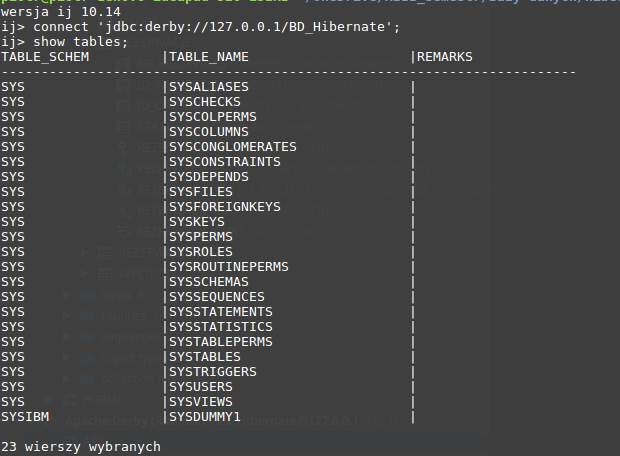
\includegraphics[scale=0.5]{I/1.png}
  \caption{Wywołanie komendy \textit{show tables} na nowo utworzonej bazie danych}
  \label{rys:1.1}
\end{figure}

\section{Klasa Product}

W~celu dodania do bazy danych tabeli \textit{Products} utworzono klasę \textit{Product}. Zawiera ona pola \textit{productID}, \textit{productName} i~\textit{unitsOnStock}. Dodano odpowiednie anotacje \ppauza @Entity, @Table ustawiającą odpowiednią nazwę tabeli, oraz @Id  dla atrybutu productID. Zapewniono także autoinkrementację klucza głównego adnotacją @GeneratedValue. Rozpatrywano możliwość ustawienia klucza głównego na pole \textit{productName}, ale utrudniałoby to ewentualne rozbudowanie modelu (przykładowo nie można by było mieć produktu dostarczanego przez różnych dostawców). Zawarto bezparametrowy konstruktor wymagany przez Hibernate do odczytywania danych oraz konstruktor paramterowy do zapisu nowych produktów w~następnym kroku. Kod klasy przedstawiono poniżej.

\begin{lstlisting}
import javax.persistence.*;

@Entity
@Table(name = "Products")
public class Product {
    @Id
    @GeneratedValue(strategy = GenerationType.AUTO)
    private int productID;
    private String productName;
    private int unitsOnStock;

    public Product() {
    }

    public Product(String productName, int unitsOnStock) {
        this.productName = productName;
        this.unitsOnStock = unitsOnStock;
    }
}
\end{lstlisting}

W~celu poprawnego zmigrowania modelu, dodano wpis do pliku konfiguracyjnego .xml, po modyfikacji ma on następującą postać:
\begin{lstlisting}[language=XML]
<?xml version='1.0' encoding='utf-8'?>
<!DOCTYPE hibernate-configuration PUBLIC
        "-//Hibernate/Hibernate Configuration DTD//EN"
        "http://www.hibernate.org/dtd/hibernate-configuration-3.0.dtd">
<hibernate-configuration>
    <session-factory>
        <property name="connection.url">jdbc:derby://127.0.0.1/BD_Hibernate</property>
        <property name="connection.driver_class">org.apache.derby.jdbc.ClientDriver</property>
        <property name="show_sql">true</property>
        <property name="format_sql">true</property>
        <property name="use_sql_comments">true</property>
        <property name="hibernate.hbm2ddl.auto">create</property>
        <mapping class="Product"></mapping>
    </session-factory>
</hibernate-configuration>
\end{lstlisting}

W~klasie Main zmodyfikowano wygenerowany automatycznie przy tworzeniu projektu z~Hibernate kod do następującej postaci:
\begin{lstlisting}
public class Main {
    private static final SessionFactory ourSessionFactory;

    static {
        try {
            Configuration configuration = new Configuration();
            configuration.configure();

            ourSessionFactory = configuration.buildSessionFactory();
        } catch (Throwable ex) {
            throw new ExceptionInInitializerError(ex);
        }
    }

    public static Session getSession() throws HibernateException {
        return ourSessionFactory.openSession();
    }

    public static void main(final String[] arg) {
        final Session session = getSession();
        Transaction tx = session.beginTransaction();
        tx.commit();
        session.close();
    }
}
\end{lstlisting}

Po uruchomieniu programu zaobserwowano tworzenie nowej tabeli (w~miejsce ewentualnej starej). Logi Hibernate'a przedstawia Rysunek~\ref{rys:2.1}. Po odświeżeniu modelu w~DataGripie widoczna jest struktura tabeli (Rysunek~\ref{rys:2.2}) dla której wygenerowano schemat (Rysunek~\ref{rys:2.3}).

\begin{figure}[ht]
  \centering
  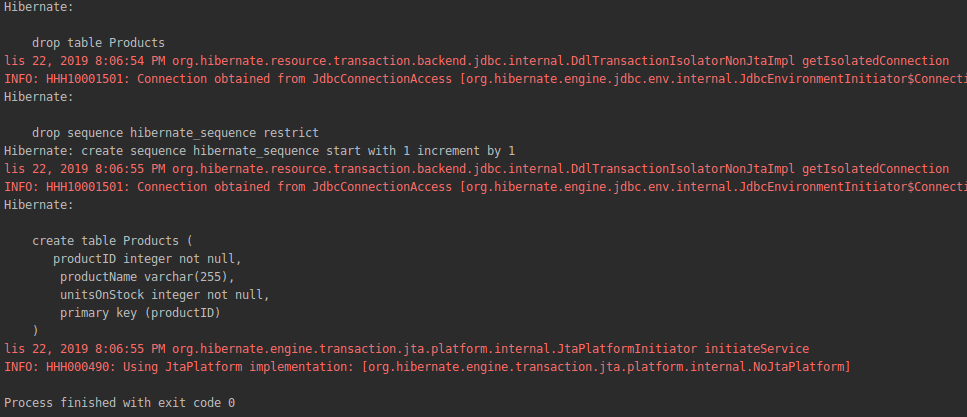
\includegraphics[width=0.9\textwidth]{II/2-1.png}
  \caption{Log Hibernate dotyczący tworzenia tabeli \textit{Products}}
  \label{rys:2.1}
\end{figure}

\begin{figure}[ht]
  \centering
  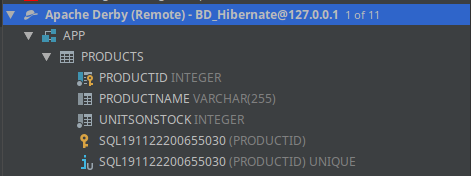
\includegraphics[scale=0.5]{II/2-2.png}
  \caption{Struktura tabeli \textit{Products} widziana w~DataGripie}
  \label{rys:2.2}
\end{figure}

\begin{figure}[ht]
  \centering
  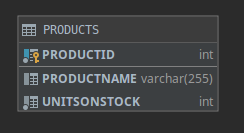
\includegraphics[scale=0.5]{II/2-3.png}
  \caption{Schemat tabeli \textit{Products} z~DataGripa}
  \label{rys:2.3}
\end{figure}

Następnie, w~celu odpytania użytkownika o~dane dodawanego produktu, zmodyfikowano funkcję main:

\begin{lstlisting}
public static void main(final String[] arg) {
	Scanner inputScanner = new Scanner(System.in);

	System.out.print("Enter product name: ");
	String productName = inputScanner.nextLine();

	System.out.print("Enter units on stock number: ");
	int unitsOnStock =  Integer.parseInt(inputScanner.nextLine());

	Product addedProduct = new Product(productName, unitsOnStock);

	final Session session = getSession();
	Transaction tx = session.beginTransaction();
	session.save(addedProduct);
	tx.commit();
	session.close();
}
\end{lstlisting}

W~konfiguracyjnym pliku .xml zmieniono ustawienie \textit{hbm2ddl.auto} z~\textit{create} na \textit{update}, aby nie usuwać starej i~nie tworzy nowej tabeli za każdym razem. Przykładowe wywołanie przedstawia Rysunek~\ref{rys:2.4}. Wynik wywołania polecenia \textit{select} na tabeli \textit{Products} potwierdzający zapis nowych danych przedstawia Rysunek~\ref{rys:2.5}.

\begin{figure}[ht]
  \centering
  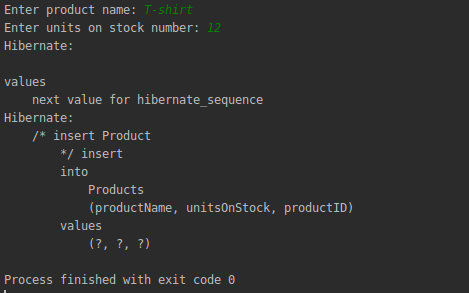
\includegraphics[scale=0.75]{II/2-4.png}
  \caption{Log Hibernate dotyczący dodania nowego wiersza do tabeli \textit{Products}}
  \label{rys:2.4}
\end{figure}

\begin{figure}[ht]
  \centering
  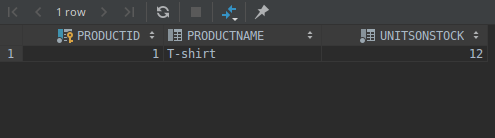
\includegraphics[scale=0.5]{II/2-5.png}
  \caption{Wynik polecenia \textit{select} wywołanego na tabeli \textit{Products}}
  \label{rys:2.5}
\end{figure}

\clearpage
\section{Klasa Supplier}

Dodano nową klasę \textit{Supplier} zawierającą pola \textit{supplierID}, \textit{companyName}, \textit{address} i~\textit{city}:

\begin{lstlisting}
import javax.persistence.*;

@Entity
@Table(name = "Suppliers")
public class Supplier {
    @Id
    @GeneratedValue(strategy = GenerationType.AUTO)
    private int supplierID;
    private String companyName;
    private String street;
    private String city;

    public Supplier() {
    }

    public Supplier(String companyName, String street, String city) {
        this.companyName = companyName;
        this.street = street;
        this.city = city;
    }
}
\end{lstlisting}

W~konfiguracyjnym pliku XML ustawiono, analogicznie jak w~poprzednim punkcie, odpowiednie mapowanie klasy. Aby utworzyć powiązanie między tabelami, do klasy Product dodano jedno nowe pole z~adnotacją @ManyToOne oraz z~dodatkowym getterem i~setterem (będą przydatne przy modyfikacji utworzonego wcześniej produktu). Dodany kod ma następującą postać:

\begin{lstlisting}
@ManyToOne
private Supplier supplier;

public void setSupplier(Supplier supplier) {
	this.supplier = supplier;
}

public Supplier getSupplier() {
	return supplier;
}
\end{lstlisting}

Zmodyfikowano funkcję main, tak aby czytano od użytkownika dane nowego dostawcy i~przypisano je do dodanego poprzednio produktu:

\begin{lstlisting}
public static void main(final String[] arg) {
	Scanner inputScanner = new Scanner(System.in);

	System.out.print("Enter company name: ");
	String companyName = inputScanner.nextLine();
	System.out.print("Enter company street: ");
	String street = inputScanner.nextLine();
	System.out.print("Enter company city: ");
	String city = inputScanner.nextLine();

	Supplier addedSupplier = new Supplier(companyName, street, city);

	final Session session = getSession();
	Transaction tx = session.beginTransaction();

	session.save(addedSupplier);
	Product firstProduct = session.get(Product.class, 1);
	firstProduct.setSupplier(addedSupplier);

	tx.commit();
	session.close();
}
\end{lstlisting}

Uruchomiono program i~dodano nowego dostawcę. Logi Hibernate przedstawia Rysunek~\ref{rys:3.1a} i~\ref{rys:3.1}, wynik wywołania polecenia \textit{select} na tabeli \textit{Products} Rysunek~\ref{rys:3.2} a~dla tabeli \textit{Suppliers} Rysunek~\ref{rys:3.3}. Stan bazy danych odczytany z~DataGripa zawiera Rysunek~\ref{rys:3.4}, a schemat bazy danych Rysunek~\ref{rys:3.5}.

\begin{figure}[ht]
  \centering
  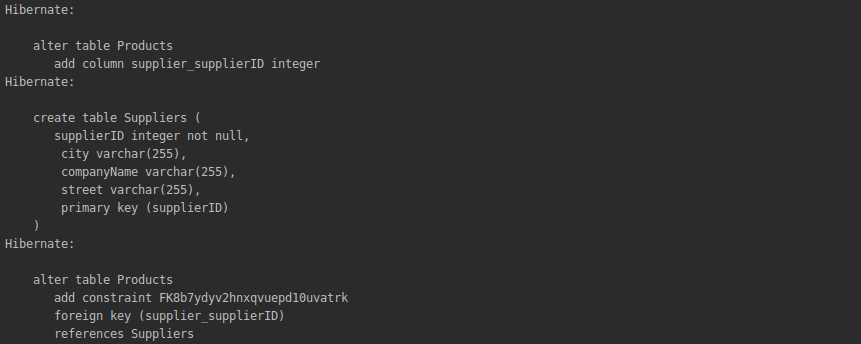
\includegraphics[width=0.75\textwidth]{III/3-1a.png}
  \caption{Log Hibernate dotyczący modyfikacji tabeli \textit{Products} i~dodania tabeli \textit{Suppliers}}
  \label{rys:3.1a}
\end{figure}

\begin{figure}[ht]
  \centering
  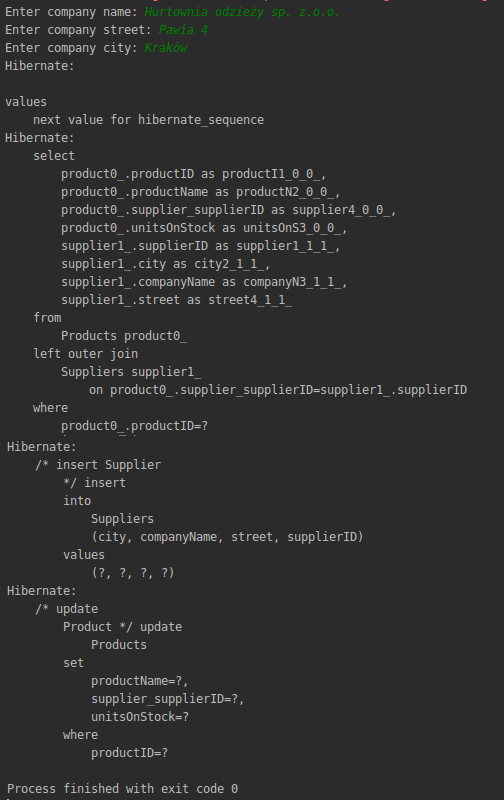
\includegraphics[scale=0.43]{III/3-1.png}
  \caption{Log Hibernate dotyczący modyfikacji danych}
  \label{rys:3.1}
\end{figure}

\begin{figure}[ht]
  \centering
  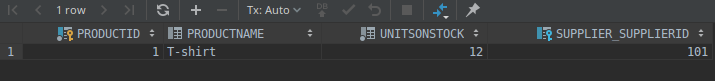
\includegraphics[scale=0.5]{III/3-2.png}
  \caption{Wynik polecenia \textit{select} wywołanego na tabeli \textit{Products}}
  \label{rys:3.2}
\end{figure}

\begin{figure}[ht]
  \centering
  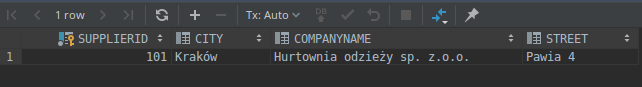
\includegraphics[scale=0.5]{III/3-3.png}
  \caption{Wynik polecenia \textit{select} wywołanego na tabeli \textit{Suppliers}}
  \label{rys:3.3}
\end{figure}

\begin{figure}[ht]
  \centering
  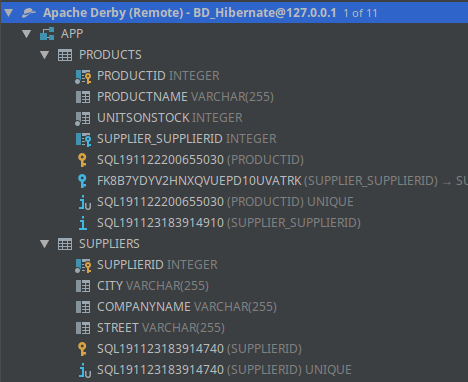
\includegraphics[scale=0.5]{III/3-4.png}
  \caption{Struktura bazy danych widziana w~DataGripie}
  \label{rys:3.4}
\end{figure}

\begin{figure}[ht]
  \centering
  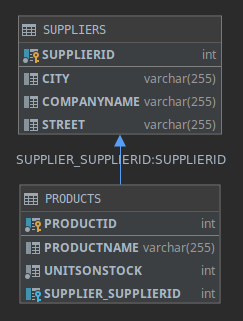
\includegraphics[scale=0.5]{III/3-5.png}
  \caption{Schemat bazy danych}
  \label{rys:3.5}
\end{figure}

\clearpage

\section{Odwrócenie relacji}

Odwrócono relację między tabelami \textit{Products} i~\textit{Suppliers} poprzez usunięcie pól dodanych do klasy Product w~poprzednim kroku i~dodaniu nowego pola do klasy Suppliers (wraz z~pomocniczą metodą):

\begin{lstlisting}
@OneToMany
private Set<Product> suppliedProducts;

public void addProductToList(Product addedProduct) {
	this.suppliedProducts.add(addedProduct);
}
\end{lstlisting}

Zmodyfikowano metodę main, tak aby czytać dane dostawcy i~produktów od użytkownika, a~następnie poprawnie je dodać do bazy danych:

\begin{lstlisting}
public static void main(final String[] arg) {
	Scanner inputScanner = new Scanner(System.in);

	System.out.print("Enter company name: ");
	String companyName = inputScanner.nextLine();
	System.out.print("Enter company street: ");
	String street = inputScanner.nextLine();
	System.out.print("Enter company city: ");
	String city = inputScanner.nextLine();

	Supplier addedSupplier = new Supplier(companyName, street, city);

	System.out.print("Enter number of supplied products: ");
	int prodNumber = Integer.parseInt(inputScanner.nextLine());

	final Session session = getSession();
	Transaction tx = session.beginTransaction();

	for(int i = 0; i < prodNumber; i++) {
		System.out.print("Enter product name: ");
		String productName = inputScanner.nextLine();
		System.out.print("Enter units on stock: ");
		int unitsOnStock = Integer.parseInt(inputScanner.nextLine());

		Product nextProduct = new Product(productName, unitsOnStock);
		session.save(nextProduct);
		addedSupplier.addProductToList(nextProduct);
	}
	session.save(addedSupplier);

	tx.commit();
	session.close();
}
\end{lstlisting}

Przed uruchomieniem programu zmodyfikowano w~pliku konfiguracyjnym parametr \textit{hbm2ddl.auto} na wartość \textit{create}. Zaobserwowano tworzenie tabeli łącznikowej \ppauza log Hibernate'a zawiera Rysunek~\ref{rys:4.1} i~\ref{rys:4.2}, wywołania polecenia \textit{select} na poszczególnych tabelach Rysunek~\ref{rys:4.3}, \ref{rys:4.4} i~\ref{rys:4.5}, strukturę bazy danych Rysunek~\ref{rys:4.6} a~schemat Rysunek~\ref{rys:4.7}.

\begin{figure}[ht]
  \centering
  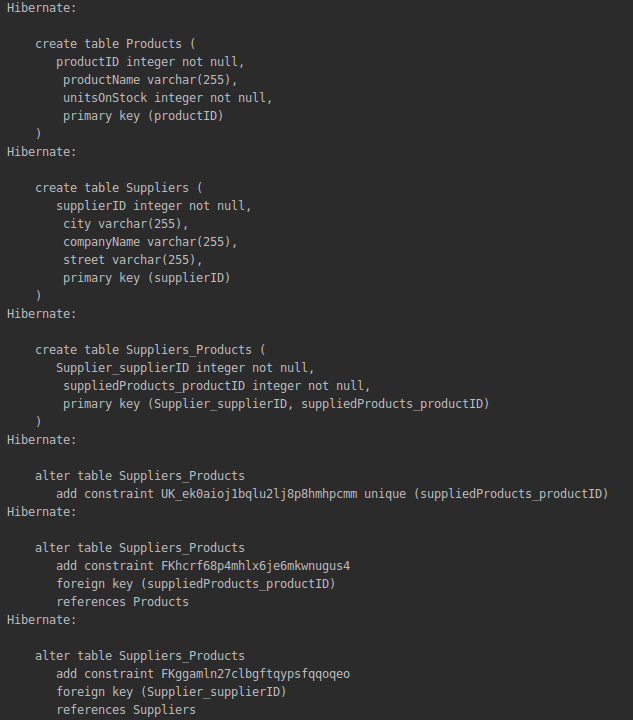
\includegraphics[width=0.75\textwidth]{IV/4-1.png}
  \caption{Log Hibernate dotyczący konstrukcji tabel z~odwróconą zależnością}
  \label{rys:4.1}
\end{figure}

\begin{figure}[ht]
  \centering
  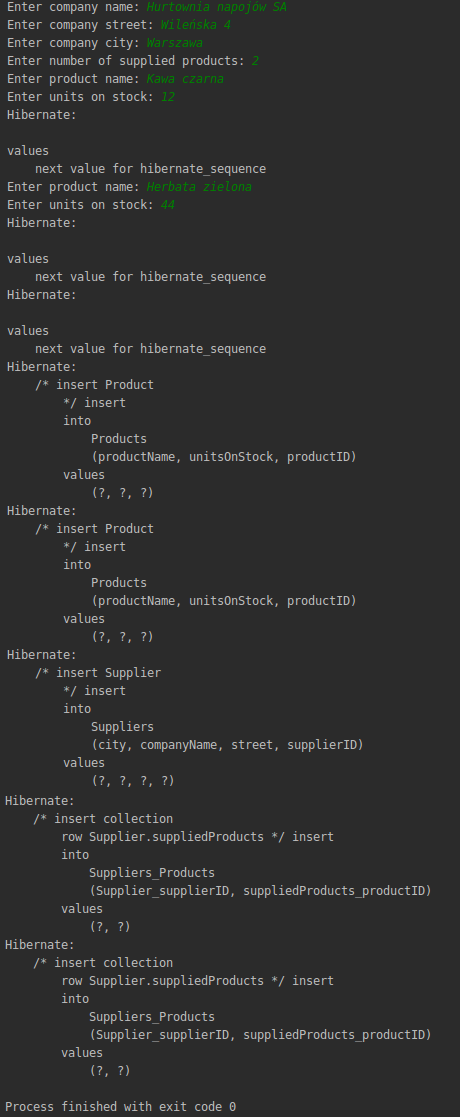
\includegraphics[width=0.55\textwidth]{IV/4-2.png}
  \caption{Log Hibernate dotyczący wstawiania nowych wartości do tabel}
  \label{rys:4.2}
\end{figure}

\begin{figure}[ht]
  \centering
  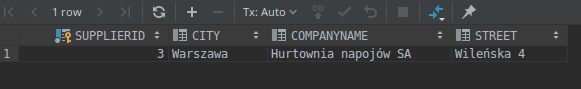
\includegraphics[scale=0.5]{IV/4-3.png}
  \caption{Wynik polecenia \textit{select} na tabeli \textit{Suppliers}}
  \label{rys:4.3}
\end{figure}

\begin{figure}[ht]
  \centering
  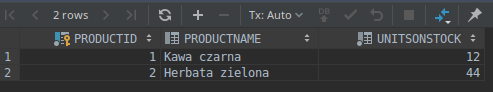
\includegraphics[scale=0.5]{IV/4-4.png}
  \caption{Wynik polecenia \textit{select} na tabeli \textit{Products}}
  \label{rys:4.4}
\end{figure}

\begin{figure}[ht]
  \centering
  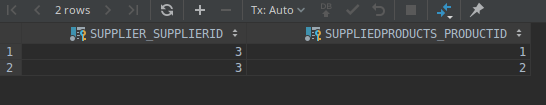
\includegraphics[scale=0.5]{IV/4-5.png}
  \caption{Wynik polecenia \textit{select} na tabeli łącznikowej}
  \label{rys:4.5}
\end{figure}

\begin{figure}[ht]
  \centering
  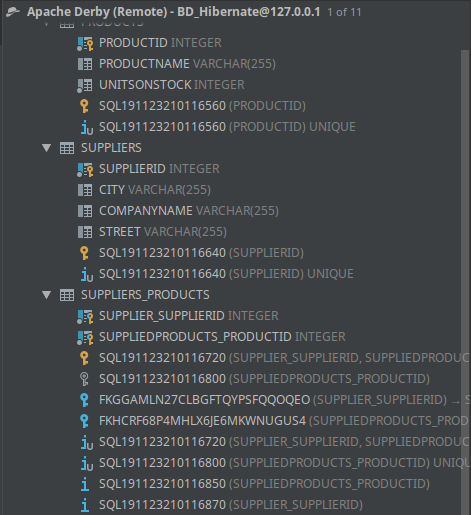
\includegraphics[scale=0.5]{IV/4-6.png}
  \caption{Struktura bazy danych widziana w~DataGripie}
  \label{rys:4.6}
\end{figure}

\clearpage
\begin{figure}[ht]
  \centering
  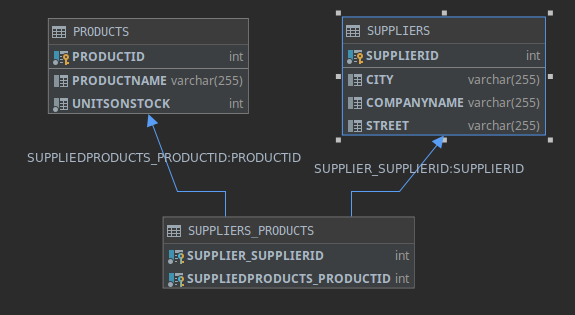
\includegraphics[scale=0.5]{IV/4-7.png}
  \caption{Schemat bazy danych}
  \label{rys:4.7}
\end{figure}

Brak tworzenia tabeli łącznikowej zapewniono dodając przed zbiorem produktów w~klasie \textit{Suppliers} adnotację @JoinColumn(name = "SUPPLIERS\_FK"). Log Hibernate'a zawarto na Rysunku~\ref{rys:4.8}, strukturę bazy danych na Rysunku~\ref{rys:4.9} a~schemat bazy danych na Rsyunku~\ref{rys:4.10}.

\begin{figure}[ht]
  \centering
  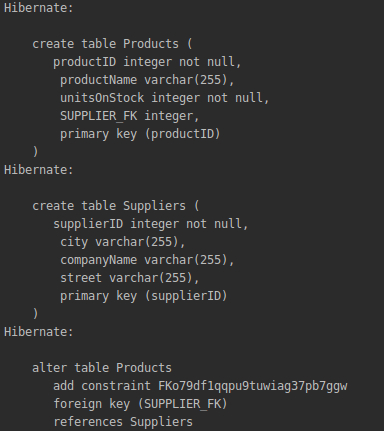
\includegraphics[scale=0.75]{IV/4-8.png}
  \caption{Log Hibernate dotyczący konstrukcji tabel z~odwróconą zależnością}
  \label{rys:4.8}
\end{figure}

\begin{figure}[ht]
  \centering
  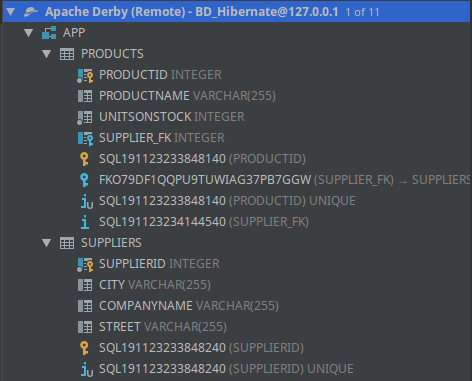
\includegraphics[scale=0.5]{IV/4-9.png}
  \caption{Struktura bazy danych widziana w~DataGripie}
  \label{rys:4.9}
\end{figure}

\begin{figure}[ht]
  \centering
  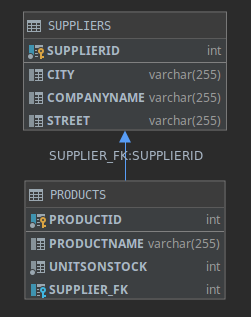
\includegraphics[scale=0.5]{IV/4-10.png}
  \caption{Schemat bazy danych}
  \label{rys:4.10}
\end{figure}

\clearpage
\section{Relacja dwukierunkowa}

Dwukierunkowość relacji zapewniono dodając atrybut supplier do klasy Product i~odpowiednio modyfikując metody ustawiające dostawcę/dodające produkt do listy dostarczanych. Klasa \textit{Product} ma następującą postać:

\begin{lstlisting}
@Entity
@Table(name = "Products")
public class Product {
    @Id
    @GeneratedValue(strategy = GenerationType.AUTO)
    private int productID;
    private String productName;
    private int unitsOnStock;
    @ManyToOne
    @JoinColumn(name = "SUPPLIER_FK")
    private Supplier supplier;

    public Product() {
    }

    public Product(String productName, int unitsOnStock) {
        this.productName = productName;
        this.unitsOnStock = unitsOnStock;
    }

    public void setSupplier(Supplier supplier) {
        this.supplier = supplier;
        this.supplier.getSuppliedProducts().add(this);
    }
}
\end{lstlisting}

a~klasa \textit{Supplier}:

\begin{lstlisting}
@Entity
@Table(name = "Suppliers")
public class Supplier {
    @Id
    @GeneratedValue(strategy = GenerationType.AUTO)
    private int supplierID;
    private String companyName;
    private String street;
    private String city;
    @OneToMany(mappedBy = "supplier")
    private Set<Product> suppliedProducts;

    public Supplier() {
    }

    public Supplier(String companyName, String street, String city) {
        this.companyName = companyName;
        this.street = street;
        this.city = city;
        this.suppliedProducts = new HashSet<>();
    }

    public void addProductToList(Product addedProduct) {
        this.suppliedProducts.add(addedProduct);
        addedProduct.setSupplier(this);
    }

    public Set<Product> getSuppliedProducts() {
        return suppliedProducts;
    }
}
\end{lstlisting}

Log Hibernate przedstawia Rysunek~\ref{rys:5.1}, wyniki wywołania \textit{select} na tabeli \textit{Suppliers} i~\textit{Products} Rysunek~\ref{rys:5.2} i~\ref{rys:5.3}, strukturę bazy danych Rysunek~\ref{rys:5.4} a~schemat bazy danych Rysunek~\ref{rys:5.5}.

\begin{figure}[ht]
  \centering
  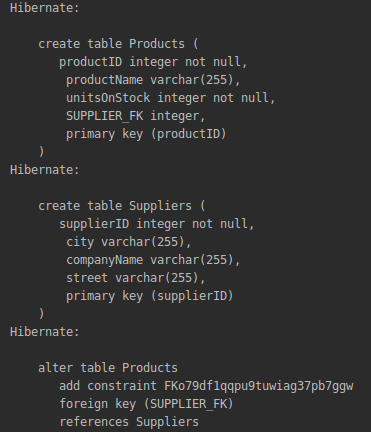
\includegraphics[scale=0.75]{V/5-1.png}
  \caption{Log Hibernate dotyczący konstrukcji tabel z~dwukierunkową zależnością}
  \label{rys:5.1}
\end{figure}

\begin{figure}[ht]
  \centering
  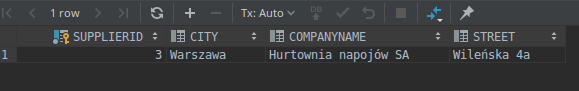
\includegraphics[scale=0.5]{V/5-2.png}
  \caption{Wynik polecenia \textit{select} na tabeli \textit{Suppliers}}
  \label{rys:5.2}
\end{figure}

\begin{figure}[ht]
  \centering
  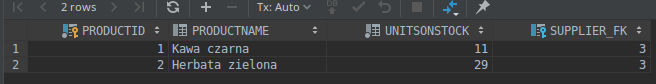
\includegraphics[scale=0.5]{V/5-3.png}
  \caption{Wynik polecenia \textit{select} na tabeli \textit{Products}}
  \label{rys:5.3}
\end{figure}

\begin{figure}[ht]
  \centering
  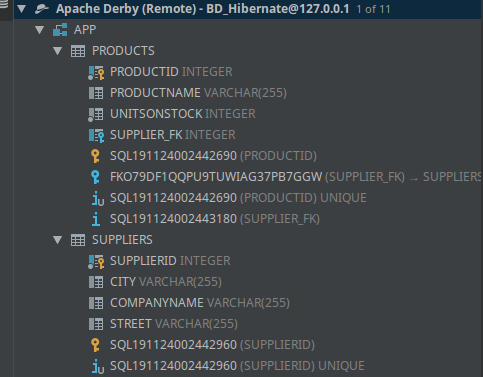
\includegraphics[scale=0.5]{V/5-4.png}
  \caption{Struktura bazy danych widziana w~DataGripie}
  \label{rys:5.4}
\end{figure}

\begin{figure}[ht]
  \centering
  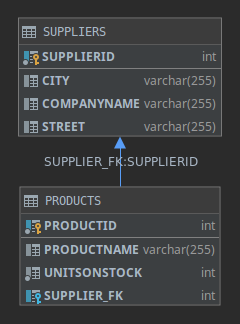
\includegraphics[scale=0.5]{V/5-5.png}
  \caption{Schemat bazy danych}
  \label{rys:5.5}
\end{figure}

\clearpage
\section{Klasa Category}

Utworzono nową klasę \textit{Category}:

\begin{lstlisting}
@Entity
@Table(name = "Categories")
public class Category {
    @Id
    @GeneratedValue(strategy = GenerationType.AUTO)
    private int categoryID;
    private String categoryName;
    @OneToMany(mappedBy = "category")
    private Set<Product> products;

    public Category() {
    }

    public Category(String categoryName) {
        this.categoryName = categoryName;
        this.products = new HashSet<>();
    }

    public void addProduct(Product product) {
        this.products.add(product);
        product.setCategory(this);
    }

    public Set<Product> getProducts() {
        return products;
    }

    @Override
    public String toString() {
        return categoryID + ": " + categoryName;
    }
}
\end{lstlisting}

Dodano także w~klasie \textit{Product} pomocnicze metody i~mapowanie relacji w~drugą stronę:

\begin{lstlisting}
@ManyToOne
@JoinColumn(name = "CATEGORY_FK")
private Category category;

public void setCategory(Category category) {
	this.category = category;
	this.category.getProducts().add(this);
}

public Category getCategory() {
	return category;
}

@Override
public String toString() {
	return productID + ": " + productName + ", unitsOnStock: " + unitsOnStock;
}
\end{lstlisting}

Logi Hibernate'a zaobserwowane przy tworzeniu nowej tabeli i~modyfikacji istniejącej (Products) przedstawia Rysunek~\ref{rys:6.1}. Strukturę bazy danych przedstawia Rysunek~\ref{rys:6.4}, a~jej schemat Rysunek~\ref{rys:6.5}. Log Hibernate'a dla dodawania nowych danych zawiera Rysunek~\ref{rys:6.2}. Po dodaniu kilku kategorii i~przypisaniu dotychczas istniejących produktów do nich, wywołano polecenie \textit{select} na tabeli \textit{Products}. Wynik zamieszczono na Rysunku~\ref{rys:6.3}.

\begin{figure}[ht]
  \centering
  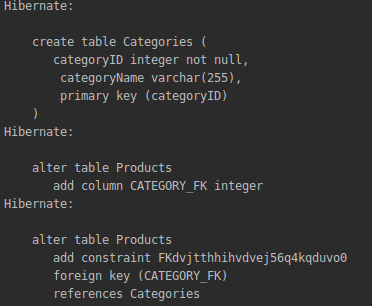
\includegraphics[scale=0.80]{VI/6-1.png}
  \caption{Log Hibernate dotyczący dodania tabeli \textit{Categories} i~modyfikacji \textit{Products}}
  \label{rys:6.1}
\end{figure}

\begin{figure}[ht]
  \centering
  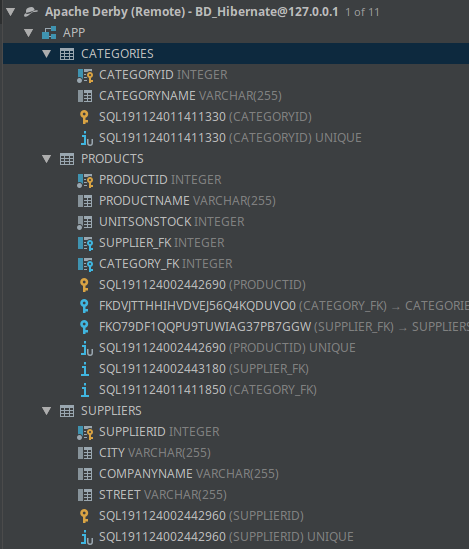
\includegraphics[scale=0.60]{VI/6-4.png}
  \caption{Struktura bazy danych widziana w~DataGripie}
  \label{rys:6.4}
\end{figure}

\begin{figure}[ht]
  \centering
  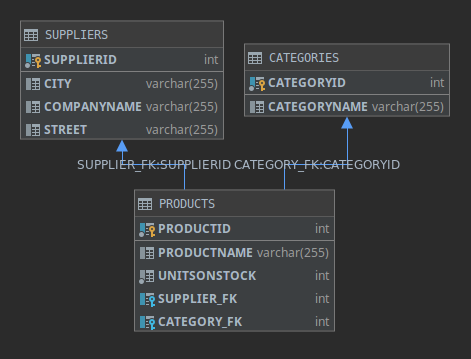
\includegraphics[scale=0.75]{VI/6-5.png}
  \caption{Schemat bazy danych}
  \label{rys:6.5}
\end{figure}

\begin{figure}[ht]
  \centering
  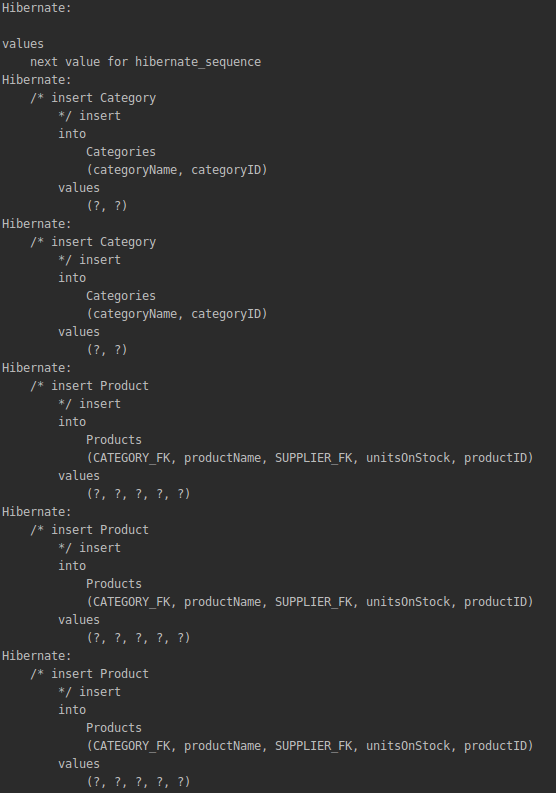
\includegraphics[width=0.75\textwidth]{VI/6-2.png}
  \caption{Log Hibernate dotyczący dodawania nowych kategorii i~produktów}
  \label{rys:6.2}
\end{figure}

\begin{figure}[ht]
  \centering
  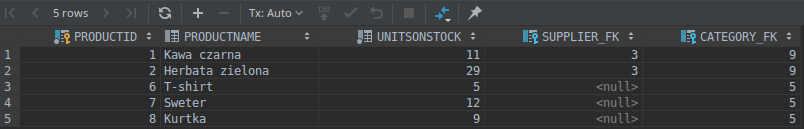
\includegraphics[scale=0.5]{VI/6-3.png}
  \caption{Wynik polecenia \textit{select} na tabeli \textit{Products}}
  \label{rys:6.3}
\end{figure}

Wyciągnięto z~poziomu maina jedną z~kategorii i~wypisano wszystkie produkty należące do niej, log przedstawia Rysunek~\ref{rys:6.6}. Następnie dla pojedynczego produktu wypisano kategorię, do której on należy \ppauza Rysunek~\ref{rys:6.7}.

\begin{figure}[ht]
  \centering
  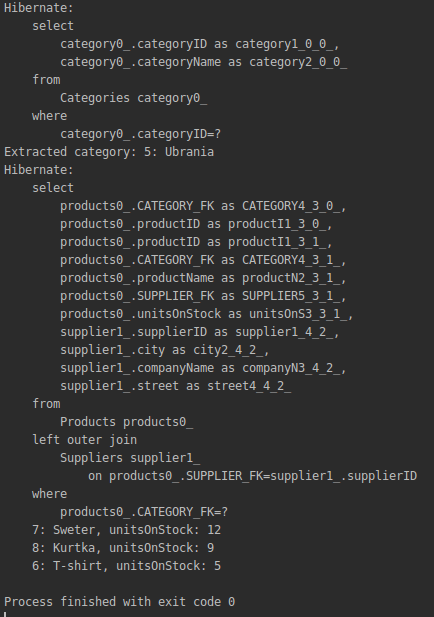
\includegraphics[width=0.65\textwidth]{VI/6-6.png}
  \caption{Log Hibernate dotyczący wyciągnięcia kategorii z~bazy i~wypisania należących do niej produktów}
  \label{rys:6.6}
\end{figure}

\begin{figure}[ht]
  \centering
  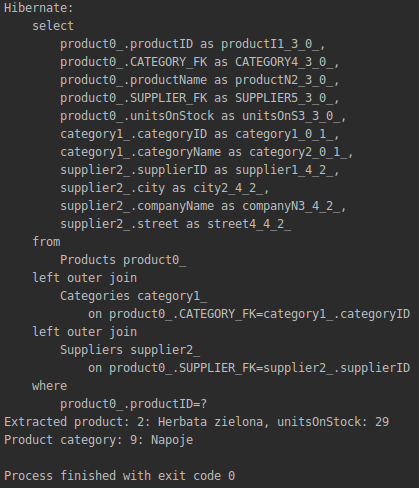
\includegraphics[width=0.65\textwidth]{VI/6-7.png}
  \caption{Log Hibernate dotyczący wyciągnięcia produktu z~bazy i~wypisania jego kategorii}
  \label{rys:6.7}
\end{figure}

\clearpage
\section{Relacja wiele\dywiz{}do\dywiz{}wielu}

Utworzono nową klasę \textit{Invoice}:

\begin{lstlisting}
@Entity
@Table(name = "Invoices")
public class Invoice {
    @Id
    @GeneratedValue(strategy = GenerationType.AUTO)
    private int invoiceNumber;
    private int quantity;
    @ManyToMany
    private Set<Product> products;

    public Invoice() {
    }

    public Invoice(int quantity) {
        this.quantity = quantity;
        this.products = new HashSet<>();
    }

    public Set<Product> getProducts() {
        return products;
    }

    public void addProduct(Product product, int quantity) {
        this.products.add(product);
        this.quantity += quantity;
        product.decreaseUnitsOnStock(quantity);
    }
}
\end{lstlisting}

Do klasy \textit{Product} dodano zbiór zamówień i~metody obsługujące zamówienia:
\begin{lstlisting}
@ManyToMany(mappedBy = "products")
private Set<Invoice> invoices;

public Set<Invoice> getInvoices() {
	return invoices;
}

public void decreaseUnitsOnStock(int quantity) {
	this.unitsOnStock -= quantity;
}
\end{lstlisting}

Po wywołaniu programu, zaobserwowano tworzenie nowej tabeli wraz z~tabelą łącznikową \ppauza log zawiera Rysunek~\ref{rys:7.1}, strukturę bazy Rysunek~\ref{rys:7.2} a~schemat bazy Rysunek~\ref{rys:7.3}. Dodano kilka zamówień, nowych produktów i~powiązano je ze sobą. Log dla wypisania produktów z~konkretnego zamówienia przedstawia Rysunek~\ref{rys:7.4}, a~dla wypisania zamówień dla konkretnego produktu Rysunek~\ref{rys:7.5}.

\begin{figure}[ht]
  \centering
  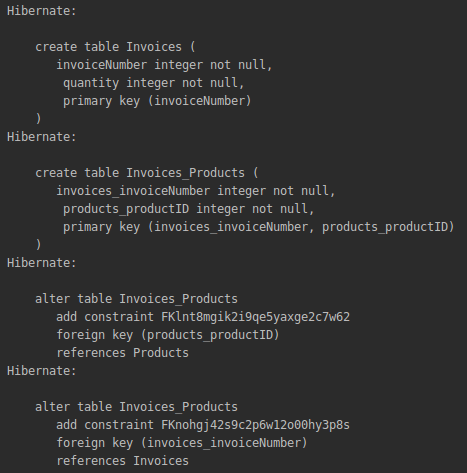
\includegraphics[scale=0.60]{VII/7-1.png}
  \caption{Log Hibernate dotyczący dodania tabeli \textit{Invoices} i~tabeli łącznikowej}
  \label{rys:7.1}
\end{figure}

\begin{figure}[ht]
  \centering
  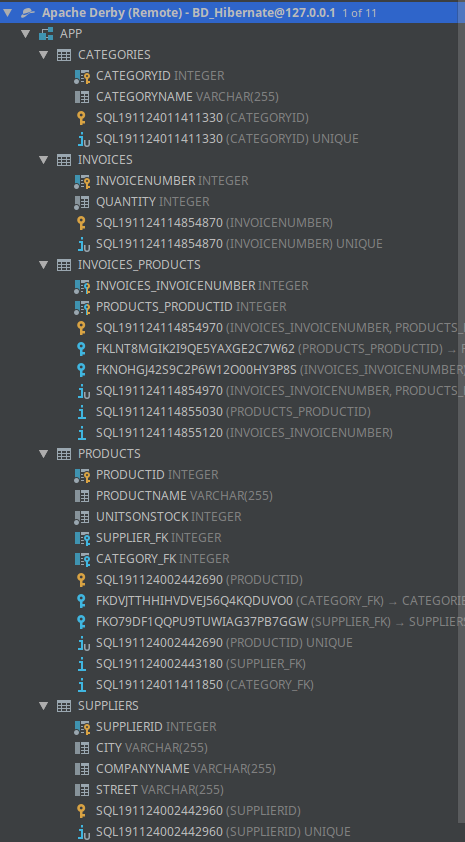
\includegraphics[scale=0.60]{VII/7-2.png}
  \caption{Struktura bazy danych widziana w~DataGripie}
  \label{rys:7.2}
\end{figure}

\begin{figure}[ht]
  \centering
  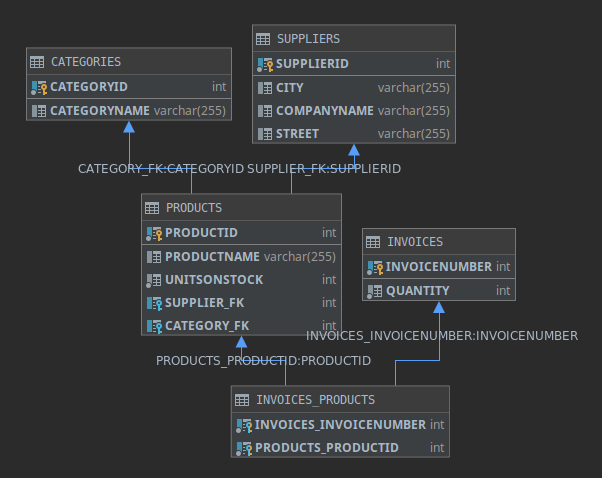
\includegraphics[scale=0.75]{VII/7-3.png}
  \caption{Schemat bazy danych}
  \label{rys:7.3}
\end{figure}

\begin{figure}[ht]
  \centering
  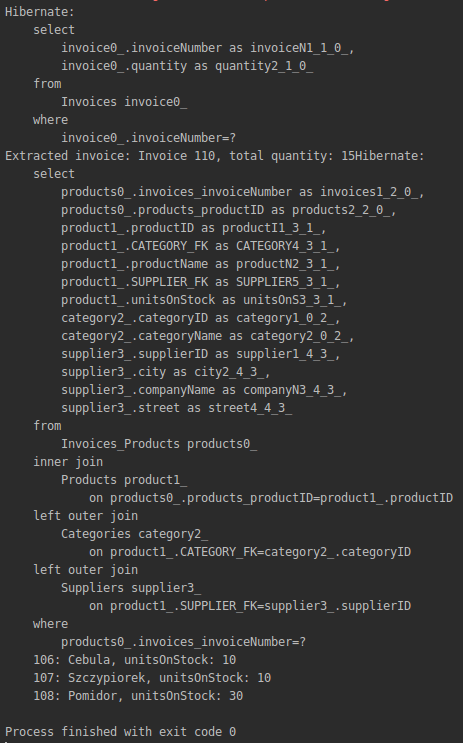
\includegraphics[width=0.65\textwidth]{VII/7-4.png}
  \caption{Log Hibernate dotyczący wyciągnięcia zamówienia z~bazy i~wypisania należących do niego produktów}
  \label{rys:7.4}
\end{figure}

\begin{figure}[ht]
  \centering
  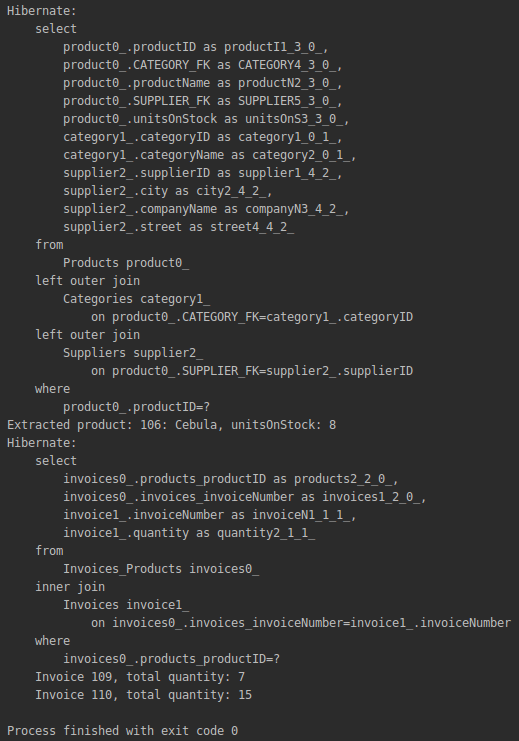
\includegraphics[width=0.65\textwidth]{VII/7-5.png}
  \caption{Log Hibernate dotyczący wyciągnięcia produktu z~bazy i~wypisania zamówień na niego}
  \label{rys:7.5}
\end{figure}

\clearpage
\section{JPA}

W~celu przejścia na korzystanie z~JPA, w~katalogu źródłowym projektu utworzono katalog META\dywiz{}INF, a~w~nim plik konfiguracyjny \textit{persistence.xml}:

\begin{lstlisting}[language=XML]
<?xml version='1.0' encoding='utf-8'?>
<persistence xmlns="http://java.sun.com/xml/ns/persistence"
             xmlns:xsi="http://www.w3.org/2001/XMLSchema-instance"
             xsi:schemaLocation="http://java.sun.com/xml/ns/persistence
        http://java.sun.com/xml/ns/persistence/persistence_2_0.xsd"
             version="2.0">
    <persistence-unit name="DBHibernateConfig"
                      transaction-type="RESOURCE_LOCAL">
        <properties>
            <property name="hibernate.connection.driver_class" 
            	value="org.apache.derby.jdbc.ClientDriver"/>
            <property name="hibernate.connection.url" value="jdbc:derby://127.0.0.1/BD_Hibernate"/>
            <property name="hibernate.show_sql" value="true"/>
            <property name="hibernate.format_sql" value="true"/>
            <property name="hibernate.hbm2ddl.auto" value="update"/>
        </properties>
    </persistence-unit>
</persistence>
\end{lstlisting}

Zdefiniowano nową klasę główną \textit{MainJPA}, w~metodzie \textit{main} utworzono dwie nowe kategorie, przypisano do istniejących produktów bez kategorii i~wypisano produkty jednej z~kategorii (Rysunek~\ref{rys:8.1}) i~kategorię jednego produktu (Rysunek~\ref{rys:8.2}), tak jak w~punkcie VI. 

Kod klasy:
\begin{lstlisting}
import javax.persistence.EntityManager;
import javax.persistence.EntityManagerFactory;
import javax.persistence.EntityTransaction;
import javax.persistence.Persistence;

public class MainJPA {
    public static void main(String[] args) {
        EntityManagerFactory emf = Persistence.createEntityManagerFactory("DBHibernateConfig");
        EntityManager em = emf.createEntityManager();
        EntityTransaction etx = em.getTransaction();
        etx.begin();

        Category foodCategory = new Category("Żywność");
        em.persist(foodCategory);

        Product food1 = em.find(Product.class, 106);
        food1.setCategory(foodCategory);
        Product food2 = em.find(Product.class, 107);
        food2.setCategory(foodCategory);
        Product food3 = em.find(Product.class, 108);
        food3.setCategory(foodCategory);

        Category washCategory = new Category("Środki czystości");
        em.persist(washCategory);

        Product washingProduct1 = em.find(Product.class, 104);
        washingProduct1.setCategory(washCategory);
        Product washingProduct2 = em.find(Product.class, 105);
        washingProduct2.setCategory(washCategory);

        Category category = em.find(Category.class, 5);
        System.out.println("Extracted category: " + category);

        for(Product nextProduct : category.getProducts()) {
            System.out.printf("\t%s\n", nextProduct);
        }

        Product product = em.find(Product.class, 2);
        System.out.println("Extracted product: " + product);
        System.out.println("Product category: " + product.getCategory());

        etx.commit();
        em.close();
    }
}
\end{lstlisting}

\begin{figure}[ht]
  \centering
  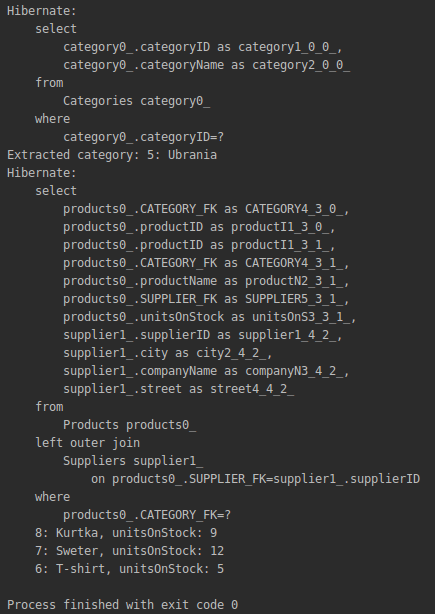
\includegraphics[width=0.65\textwidth]{VIII/8-1.png}
  \caption{Log Hibernate dotyczący wyciągnięcia kategorii z~bazy i~wypisania należących do niej produktów}
  \label{rys:8.1}
\end{figure}

\begin{figure}[ht]
  \centering
  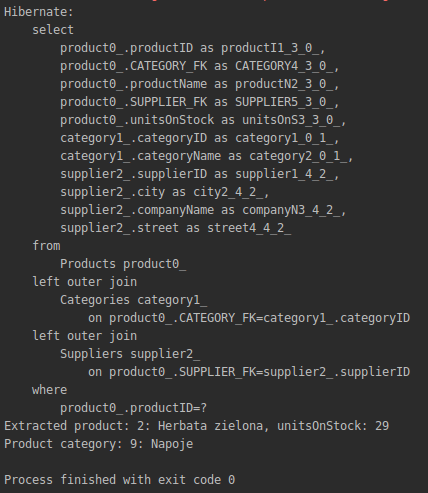
\includegraphics[width=0.65\textwidth]{VIII/8-2.png}
  \caption{Log Hibernate dotyczący wyciągnięcia produktu z~bazy i~wypisania jego kategorii}
  \label{rys:8.2}
\end{figure}

\clearpage
\section{Kaskady}

W~klasie \textit{Invoices} zmieniono adnotację przed zbiorem produktów na:
\begin{lstlisting}
@ManyToMany(cascade = {CascadeType.PERSIST})
private Set<Product> products;
\end{lstlisting}

analogicznie w~klasie \textit{Product}:
\begin{lstlisting}
@ManyToMany(mappedBy = "products", cascade = CascadeType.PERSIST)
private Set<Invoice> invoices;
\end{lstlisting}

Po wywołaniu funkcji \textit{main}:
\begin{lstlisting}
public static void main(String[] args) {
	EntityManagerFactory emf = Persistence.createEntityManagerFactory("DBHibernateConfig");
	EntityManager em = emf.createEntityManager();
	EntityTransaction etx = em.getTransaction();
	etx.begin();

	Invoice newInvoice = new Invoice(0);
	Product product1 = new Product("Paluszki solone", 3);
	Product product2 = new Product("Orzeszki ziemne", 5);

	newInvoice.addProduct(product1, 1);
	newInvoice.addProduct(product2, 3);

	em.persist(newInvoice);

	Product newProduct = new Product("Piłka do siatkówki", 20);

	Invoice invoice1 = new Invoice(0);
	Invoice invoice2 = new Invoice(0);

	newProduct.addInvoice(invoice1, 2);
	newProduct.addInvoice(invoice2, 5);

	em.persist(newProduct);

	etx.commit();
	em.close();
}
\end{lstlisting}

Zaobserwowano dodawanie wszystkich utworzonych elementów. Wynik wywołania \textit{select} na tabeli \textit{Products} przedstawia Rysunek~\ref{rys:9.1}, na tabeli łącznikowej Rysunek~\ref{rys:9.2}. Faktury utworzone w~drugiej części programu (dodane do zbioru wewnątrz produktu) nie są mapowane do tabeli łącznikowej, ze względu na to, że właścicielem tej tabeli jest klasa \textit{Invoice} a~nie \textit{Products}.

\begin{figure}[ht]
  \centering
  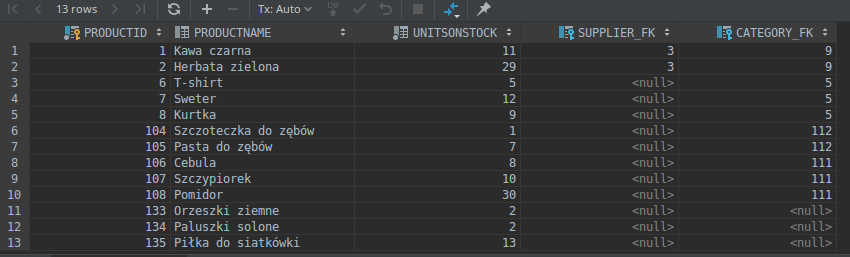
\includegraphics[scale=0.5]{IX/9-1.png}
  \caption{Wynik polecenia \textit{select} na tabeli \textit{Products}}
  \label{rys:9.1}
\end{figure}

\begin{figure}[ht]
  \centering
  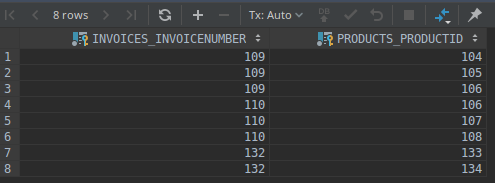
\includegraphics[scale=0.5]{IX/9-2.png}
  \caption{Wynik polecenia \textit{select} na tabeli łącznikowej}
  \label{rys:9.2}
\end{figure}

\clearpage
\section{Embedded class}

Utworzono nową klasę \textit{Address}:
\begin{lstlisting}
@Embeddable
public class Address {
    private String street;
    private String city;
    private String postalCode;
    private String country;

    public Address() {
    }

    public Address(String street, String city, String postalCode, String country) {
        this.street = street;
        this.city = city;
        this.postalCode = postalCode;
        this.country = country;
    }
}
\end{lstlisting}

W~klasie \textit{Suppliers} dodano nowy atrybut w~zamian za poprzednie odpowiadające adresowi:
\begin{lstlisting}
@Entity
@Table(name = "Suppliers")
public class Supplier {
    @Id
    @GeneratedValue(strategy = GenerationType.AUTO)
    private int supplierID;
    private String companyName;
    @Embedded
    private Address address;
    @OneToMany(mappedBy = "supplier")
    private Set<Product> suppliedProducts;

    public Supplier() {
    }

    public Supplier(String companyName, String street, String postalCode, String city, String country){
        this.companyName = companyName;
        this.address = new Address(street, city, postalCode, country);

        this.suppliedProducts = new HashSet<>();
    }

    public void addProductToList(Product addedProduct) {
        this.suppliedProducts.add(addedProduct);
        addedProduct.setSupplier(this);
    }

    public Set<Product> getSuppliedProducts() {
        return suppliedProducts;
    }
}
\end{lstlisting}

Po uruchomieniu programu zaobserwowano dodawanie nowych kolumn do tabeli \textit{Suppliers}. Log Hibernate'a przedstawia Rysunek~\ref{rys:10.1} a~schemat bazy danych Rysunek~\ref{rys:10.2}.

\begin{figure}[ht]
  \centering
  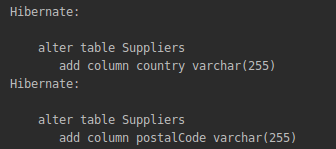
\includegraphics[scale=0.5]{X/10-1.png}
  \caption{Log Hibernate dotyczący dodawania nowych kolumn}
  \label{rys:10.1}
\end{figure}

\begin{figure}[ht]
  \centering
  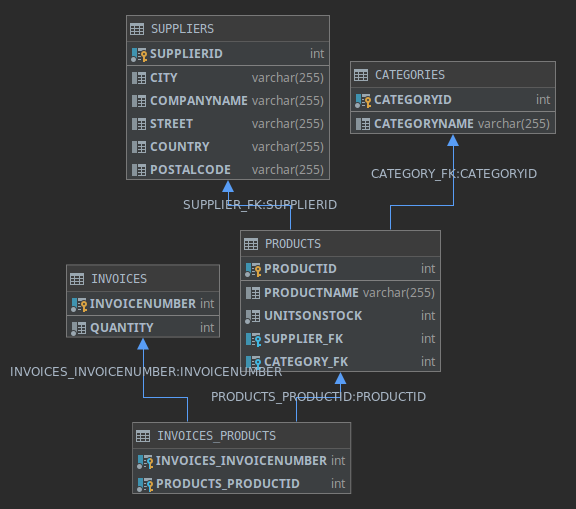
\includegraphics[scale=0.5]{X/10-2.png}
  \caption{Schemat bazy danych}
  \label{rys:10.2}
\end{figure}

\newpage
Zmodyfikowano klasę \textit{Supplier} tak, aby była mapowana do dwóch tabel:
\begin{lstlisting}
@Entity
@Table(name = "Suppliers")
@SecondaryTable(name = "Address")
public class Supplier {
    @Id
    @GeneratedValue(strategy = GenerationType.AUTO)
    private int supplierID;
    private String companyName;
    @Column(table = "Address")
    private String street;
    @Column(table = "Address")
    private String postalCode;
    @Column(table = "Address")
    private String city;
    @Column(table = "Address")
    private String country;
    @OneToMany(mappedBy = "supplier")
    private Set<Product> suppliedProducts;

    public Supplier() {
    }

    public Supplier(String companyName, String street, String postalCode, String city, String country){
        this.companyName = companyName;
        this.street = street;
        this.postalCode = postalCode;
        this.city = city;
        this.country = country;

        this.suppliedProducts = new HashSet<>();
    }

    public void addProductToList(Product addedProduct) {
        this.suppliedProducts.add(addedProduct);
        addedProduct.setSupplier(this);
    }

    public Set<Product> getSuppliedProducts() {
        return suppliedProducts;
    }
}
\end{lstlisting}

Log Hibernate'a załączono na Rysunku~\ref{rys:10.3}, a~schemat bazy danych na Rysunku~\ref{rys:10.4}.

\begin{figure}[ht]
  \centering
  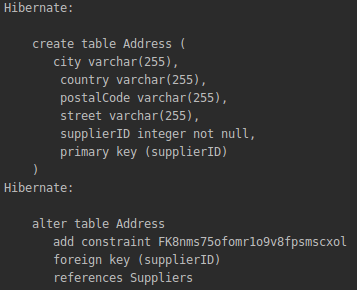
\includegraphics[scale=0.5]{X/10-3.png}
  \caption{Log Hibernate dotyczący mapowania klasy \textit{Supplier} do dwóch różnych tabel}
  \label{rys:10.3}
\end{figure}

\begin{figure}[ht]
  \centering
  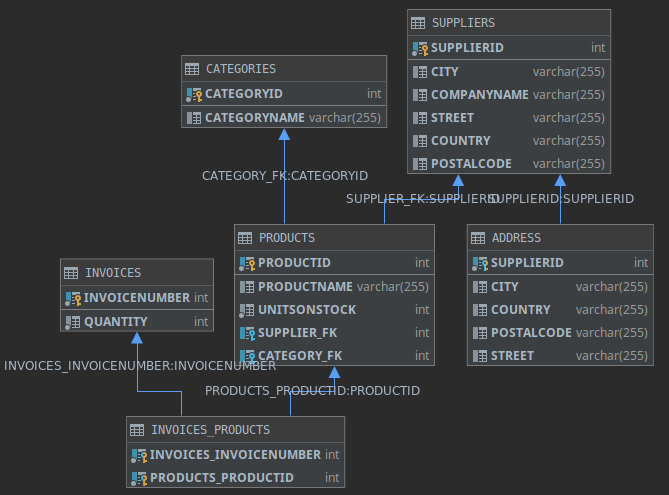
\includegraphics[scale=0.5]{X/10-4.png}
  \caption{Schemat bazy danych}
  \label{rys:10.4}
\end{figure}

\clearpage
\section{Dziedziczenie}

\subsection{Jedna tabela na całą hierarchię}

Utworzono abstrakcjną klasę \textit{Company}:
\begin{lstlisting}
@Entity
@Table(name = "Companies")
@SecondaryTable(name = "Address")
@Inheritance(strategy = InheritanceType.SINGLE_TABLE)
public abstract class Company {
    @Id
    @GeneratedValue(strategy = GenerationType.AUTO)
    private int companyID;
    private String companyName;
    @Column(table = "Address")
    private String street;
    @Column(table = "Address")
    private String postalCode;
    @Column(table = "Address")
    private String city;
    @Column(table = "Address")
    private String country;

    public Company() {
    }

    public Company(String companyName, String street, String postalCode, String city, String country) {
        this.companyName = companyName;
        this.street = street;
        this.postalCode = postalCode;
        this.city = city;
        this.country = country;
    }
    
    @Override
    public String toString() {
        return "Company name: " + companyName
                + ", address: "
                + street + " " + postalCode
                + " " + city + ", " + country;
    }
}
\end{lstlisting}

Zmodyfikowana klasa \textit{Supplier} ma postać:
\begin{lstlisting}
@Entity
@DiscriminatorValue(value = "S")
public class Supplier extends Company {
    private String bankAccountNumber;
    @OneToMany(mappedBy = "supplier")
    private Set<Product> suppliedProducts;

    public Supplier() {
        super();
    }

    public Supplier(String companyName, String street, String postalCode, String city, String country, 
    	String bankAccountNumber) {
        super(companyName, street, postalCode, city, country);

        this.bankAccountNumber = bankAccountNumber;
        this.suppliedProducts = new HashSet<>();
    }

    public void addProductToList(Product addedProduct) {
        this.suppliedProducts.add(addedProduct);
        addedProduct.setSupplier(this);
    }

    public Set<Product> getSuppliedProducts() {
        return suppliedProducts;
    }
    
    @Override
    public String toString() {
        return super.toString() 
                + ", bank account number: " + bankAccountNumber;
    }
}
\end{lstlisting}

a~nowa klasa \textit{Customer}:
\begin{lstlisting}
@Entity
@DiscriminatorValue(value = "C")
public class Customer extends Company {
    private double discount;

    public Customer() {
        super();
    }

    public Customer(String companyName, String street, String postalCode, String city, String country, 
    	double discount) {
        super(companyName, street, postalCode, city, country);

        this.discount = discount;
    }

    public double getDiscount() {
        return discount;
    }

    public void setDiscount(double discount) {
        this.discount = discount;
    }
    
    @Override
    public String toString() {
        return super.toString()
                + ", discount: " + discount;
    }
}
\end{lstlisting}

Log dla operacji tworzenia tabel zawiera Rysunek~\ref{rys:11.1}, schemat bazy danych Rysunek~\ref{rys:11.2}, a~wynik polecenia \textit{select} na tabeli \textit{Companies} Rysunek~\ref{rys:11.3}.

\begin{figure}[ht]
  \centering
  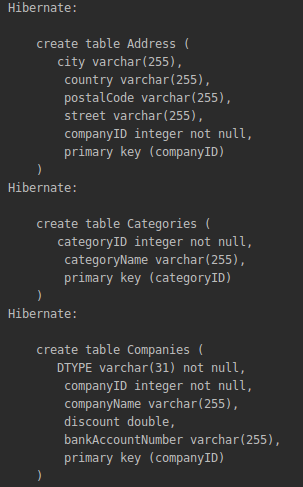
\includegraphics[scale=0.5]{XI/11-1.png}
  \caption{Log Hibernate dotyczący tworzenia nowych tabel w~hierarchii dziedziczenia}
  \label{rys:11.1}
\end{figure}

\begin{figure}[ht]
  \centering
  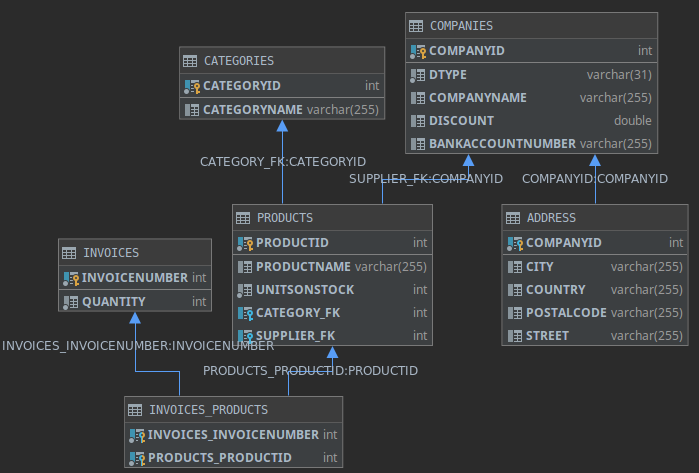
\includegraphics[scale=0.40]{XI/11-2.png}
  \caption{Schemat bazy danych}
  \label{rys:11.2}
\end{figure}

\begin{figure}[ht]
  \centering
  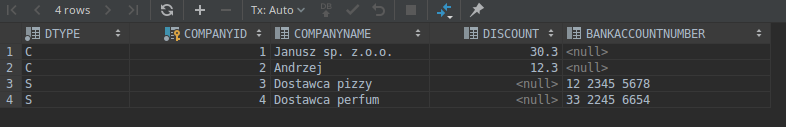
\includegraphics[scale=0.5]{XI/11-3.png}
  \caption{Wynik polecenia \textit{select} na tabeli \textit{Companies}}
  \label{rys:11.3}
\end{figure}

Wypisano wszystkich klientów korzystając z~kodu (wynik przedstawia Rysunek~\ref{rys:11.4}):
\begin{lstlisting}
List<Customer> customers = em.createQuery("from Customer").getResultList();
for(Customer c : customers) {
	System.out.println(c);
}
\end{lstlisting}

\begin{figure}[ht]
  \centering
  \includegraphics[scale=0.5]{XI/11-4.png}
  \caption{Wynik wypisania wszystkich klientów}
  \label{rys:11.4}
\end{figure}

\clearpage
\subsection{Tabele łączone}

Zmieniono adnotację stojącą przed deklaracją klasy \textit{Company} na @Inheritance(strategy = InheritanceType.JOINED), usunięto adnotacje @DiscriminatorValue i~dodano adnotacje @Table do klas \textit{Supplier} i~\textit{Customer} określające nazwy tabel. Dalej wykonano analogiczne kroki jak w~poprzednim podpunkcie. Log dla operacji tworzenia tabel zawiera Rysunek~\ref{rys:11.5}, schemat bazy danych Rysunek~\ref{rys:11.6}, wynik polecenia \textit{select} na tabeli \textit{Companies} Rysunek~\ref{rys:11.7}, a~wynik wypisania wszystkich klientów Rysunek~\ref{rys:11.8}.

\begin{figure}[ht]
  \centering
  \includegraphics[scale=0.5]{XI/11-5.png}
  \caption{Log Hibernate dotyczący tworzenia nowych tabel w~hierarchii dziedziczenia}
  \label{rys:11.5}
\end{figure}

\begin{figure}[ht]
  \centering
  \includegraphics[scale=0.45]{XI/11-6.png}
  \caption{Schemat bazy danych}
  \label{rys:11.6}
\end{figure}

\begin{figure}[ht]
  \centering
  \includegraphics[scale=0.5]{XI/11-7.png}
  \caption{Wynik polecenia \textit{select} na tabeli \textit{Companies}}
  \label{rys:11.7}
\end{figure}

\begin{figure}[ht]
  \centering
  \includegraphics[scale=0.5]{XI/11-8.png}
  \caption{Wynik wypisania wszystkich klientów}
  \label{rys:11.8}
\end{figure}

\clearpage
\subsection{Jedna tabela na klasę}

Zmieniono adnotację stojącą przed deklaracją klasy \textit{Company} na @Inheritance(strategy = InheritanceType.TABLE\_PER\_CLASS). Usunięto z~tej klasy adnotacje służące do tworzenia osobnej tabeli na adresy. Dalej wykonano analogiczne kroki jak w~poprzednim podpunkcie. Log dla operacji tworzenia tabel zawiera Rysunek~\ref{rys:11.9}, schemat bazy danych Rysunek~\ref{rys:11.10}, wynik polecenia \textit{select} na tabeli \textit{Companies} Rysunek~\ref{rys:11.11}, a~wynik wypisania wszystkich klientów Rysunek~\ref{rys:11.12}.

\begin{figure}[ht]
  \centering
  \includegraphics[scale=0.5]{XI/11-9.png}
  \caption{Log Hibernate dotyczący tworzenia nowych tabel w~hierarchii dziedziczenia}
  \label{rys:11.9}
\end{figure}

\begin{figure}[ht]
  \centering
  \includegraphics[scale=0.45]{XI/11-10.png}
  \caption{Schemat bazy danych}
  \label{rys:11.10}
\end{figure}

\begin{figure}[ht]
  \centering
  \includegraphics[scale=0.5]{XI/11-11.png}
  \caption{Wynik polecenia \textit{select} na tabeli \textit{Companies}}
  \label{rys:11.11}
\end{figure}

\begin{figure}[ht]
  \centering
  \includegraphics[scale=0.5]{XI/11-12.png}
  \caption{Wynik wypisania wszystkich klientów}
  \label{rys:11.12}
\end{figure}

\clearpage
\section{Aplikacja do zamawiania produktów}

Do aplikacji dodano klasy odpowiedzialne za wyświetlanie menu konsolowego (Menu) i~logowania (Logger):

\begin{lstlisting}
import javax.persistence.EntityManager;
import javax.persistence.EntityTransaction;
import javax.persistence.TypedQuery;
import java.util.List;
import java.util.Scanner;

public class Logger {
    private EntityManager em;
    private Scanner scanner;

    public Logger(EntityManager em, Scanner scanner) {
        this.em = em;
        this.scanner = scanner;
    }

    public Customer loginCompany() {
        System.out.println("Hello to Java Hibernate App.");
        System.out.printf("\tL - log in as an existing user\n\tR - create new account\n");
        System.out.printf("\tAny other key - exit\n");
        System.out.print("Response: ");
        String resp = scanner.nextLine().toLowerCase();

        if (resp.equals("l")) {
            return authenticateUser();
        } else if (resp.equals("r")) {
            return createNewUser();
        } else {
            return null;
        }
    }

    private Customer authenticateUser() {
        System.out.print("\tCompany name: ");
        String companyName = scanner.nextLine();

        TypedQuery<Customer> companyQuery = em.createQuery("from Customer 
        	as customer where customer.companyName = :compName", Customer.class);
        companyQuery.setParameter("compName", companyName);

        List<Customer> result = companyQuery.getResultList();
        if (result.size() != 1) {
            System.out.println("Authentication failed");
            System.exit(1);
        }

        System.out.println("Authentication successfull");
        return result.get(0);

    }

    private Customer createNewUser() {
        System.out.print("Enter company name: ");
        String companyName = scanner.nextLine();

        TypedQuery<Customer> companyQuery = em.createQuery("from Customer 
        	as company where company.companyName = :compName", Customer.class);
        companyQuery.setParameter("compName", companyName);

        List<Customer> result = companyQuery.getResultList();
        if (result.size() != 0) {
            System.out.println("Company with this name already exists!");
            System.exit(1);
        }

        System.out.print("Company street: ");
        String street = scanner.nextLine();
        System.out.print("Company postal code: ");
        String postalCode = scanner.nextLine();
        System.out.print("Company city: ");
        String city = scanner.nextLine();
        System.out.print("Company country: ");
        String country = scanner.nextLine();

        Customer registrationResult = new Customer(companyName, 
        	street, postalCode, city, country, 0.0);

        EntityTransaction etx = em.getTransaction();
        etx.begin();
        em.persist(registrationResult);
        etx.commit();
        ;

        return registrationResult;
    }
}
\end{lstlisting}

\begin{lstlisting}
import java.util.HashMap;
import java.util.Scanner;
import java.util.function.Consumer;

public class Menu {
    private String entryText;
    private HashMap<Integer, MenuEntry> options;
    private Integer index;
    private boolean continueAction = true;

    public Menu(String entryText) {
        this.entryText = entryText;
        this.index = new Integer(1);
        this.options = new HashMap<>();
    }

    public void addOption(String description, Consumer<Scanner> action) {
        this.options.put(this.index, new MenuEntry(description, action));
        this.index += 1;
    }

    public void display() {
        System.out.println(this.entryText);

        Scanner inputScanner = new Scanner(System.in);
        while (this.continueAction) {
            for (int i = 1; i < index; i++) {
                System.out.printf("%d - %s\n", i, this.options.get(i).getDescription());
            }

            System.out.print("Enter option number: ");
            Integer chosenOption = Integer.parseInt(inputScanner.nextLine());

            if (this.options.containsKey(chosenOption)) {
                this.options.get(chosenOption).getEntryAction().accept(inputScanner);
            } else {
                System.out.println("Wrong action!");
            }
        }

    }
}
\end{lstlisting}

Wykorzystywana jest także pomocnicza klasa MenuEntry:

\begin{lstlisting}
import java.util.Scanner;
import java.util.function.Consumer;

public class MenuEntry {
    private String description;
    private Consumer<Scanner> entryAction;

    public MenuEntry(String description, Consumer<Scanner> entryAction) {
        this.description = description;
        this.entryAction = entryAction;
    }

    public String getDescription() {
        return description;
    }

    public Consumer<Scanner> getEntryAction() {
        return entryAction;
    }
}
\end{lstlisting}

W~głównym programie uruchamiany jest mechanizm logowania/rejestracji nowego użytkownika, a~następnie menu z~opcjami: obejrzenia zamówień i~złożenia nowego zamówienia:
\begin{lstlisting}
import javax.persistence.*;
import java.util.LinkedList;
import java.util.List;
import java.util.Scanner;

public class MainApp {
    public static Customer loggedUser;
    public static EntityManager em;

    public static void main(String[] args) {
        EntityManagerFactory emf = Persistence.createEntityManagerFactory("DBHibernateConfig");
        em = emf.createEntityManager();

        Scanner inputScanner = new Scanner(System.in);
        Logger logger = new Logger(em, inputScanner);
        loggedUser = logger.loginCompany();

        Menu menu;

        menu = new Menu("Hello customer");
        menu.addOption("show orders", MainApp::listOrders);
        menu.addOption("make new order", MainApp::makeNewOrder);
        menu.addOption("exit", x -> System.exit(0));
        menu.display();

        em.close();
    }

    public static void listOrders(Scanner scanner) {
        for (Invoice currentInvoice : loggedUser.getInvoices()) {
            System.out.println("Order number: " + currentInvoice.getInvoiceNumber());
            System.out.printf("Quantity: " + currentInvoice.getQuantity());
            for (Product invoiceProduct : currentInvoice.getProducts()) {
                System.out.printf("\t%s\n", invoiceProduct.getProductName());
            }
        }
    }

    public static void listProducts() {
        TypedQuery<Product> query = em.createQuery("from Product", Product.class);
        List<Product> products = query.getResultList();

        System.out.printf("ID\t\tNAME\t\tUNITS ON STOCK\n");
        for (Product currentProduct : products) {
            System.out.printf("%d\t\t%s\t\t%d\n", currentProduct.getProductID(), 
            	currentProduct.getProductName(), currentProduct.getUnitsOnStock());
        }
    }

    public static void makeNewOrder(Scanner scanner) {
        Invoice newInvoice = new Invoice(0);
        listProducts();
        boolean continueReading = true;

        EntityTransaction etx = em.getTransaction();
        etx.begin();

        while (continueReading) {
            System.out.print("Enter product number: ");
            Integer productNumber = Integer.parseInt(scanner.nextLine());
            System.out.print("Enter quantity: ");
            Integer quantity = Integer.parseInt(scanner.nextLine());

            Product orderedProduct = em.find(Product.class, productNumber);
            if (quantity <= orderedProduct.getUnitsOnStock()) {
                newInvoice.addProduct(orderedProduct, quantity);
            } else {
                System.out.println("Given number is bigger than units on stock number!");
            }

            System.out.println("End order? (Y/N)");
            String response = scanner.nextLine().toLowerCase();

            if (response.equals("y")) {
                continueReading = false;
            }
        }

        em.persist(newInvoice);
        loggedUser.addInvoice(newInvoice);

        etx.commit();
    }
}
\end{lstlisting}

Przypadek użycia dla istniejącego użytkownika przedstawia Rysunek~\ref{rys:12.1}, a~dla rejestracji nowego Rysunek~\ref{rys:12.2}.

\begin{figure}[ht]
  \centering
  \includegraphics[scale=0.7]{XII/12-1.png}
  \caption{Przypadek użycia dla zarejestrowanego użytkownika}
  \label{rys:12.1}
\end{figure}

\begin{figure}[ht]
  \centering
  \includegraphics[scale=0.7]{XII/12-2.png}
  \caption{Przypadek użycia dla rejestracji nowego użytkownika}
  \label{rys:12.2}
\end{figure}

\end{document}